% !TEX program = xelatex
\documentclass[UTF8,zihao=-4]{oucart}
\usepackage{indentfirst}
\usepackage{graphicx}
\usepackage{caption}
\usepackage{subfigure}
\usepackage{hyperref}
\usepackage{booktabs}
\usepackage{tikz}
\usetikzlibrary{positioning,decorations.pathreplacing}
\usepackage{ctex}
\setmainfont{Times New Roman}
\usepackage[sort&compress]{natbib}
\usepackage{gbt7714}
\usepackage{amsmath}
\usepackage{amssymb}
\usepackage{algorithm}
\usepackage{algorithmic}
\usepackage{array}
\usepackage{multirow}

\makeatletter
\renewcommand\@cite[1]{{\textsuperscript{[{#1}]}}}
\makeatother

\title{基于GPU的三矩阵融合乘法研究（模板示例）}
\entitle{Template Example for GPU Triple-Matrix Fusion}
\author{你的姓名}
\studentid{你的学号}
\advisor{指导教师}
\department{学院名称}{专业班级}

\cnabstractkeywords{
    本模板用于展示中国海洋大学本科毕业论文的基础版式。正文只保留少量“三矩阵链式乘法融合优化”相关示例内容，用于演示章节层级、公式、图表、表格与参考文献的排版效果。实际使用时，建议保留当前模板结构，再将各章节内容替换为自己的论文正文。
}
{
    三矩阵乘法；GPU；论文模板；LaTeX 排版
}
\enabstractkeywords{
    This template demonstrates the basic layout for an undergraduate thesis at Ocean University of China. Only a small amount of content related to triple matrix fusion multiplication is kept as placeholder text so that sections, equations, figures, tables, and references can be previewed during writing.
}{
    triple matrix multiplication; GPU; thesis template; LaTeX
}

\begin{document}

    \makecover
    \makesignature
    \makeabstract

    \pagestyle{tableofcontents}
    \tableofcontents
    \clearpage
    \pagestyle{mainbody}

    \pagenumbering{arabic}
    \setcounter{page}{1}

    \section{绪论}

\subsection{研究背景与意义}

矩阵乘法是高性能计算和深度学习中的基础操作。为了展示论文模板的章节层级与正文样式，本模板选取三矩阵链式乘法
\[
\mathbf{M} = \mathbf{X}\mathbf{A}\mathbf{B}
\]
作为示例主题，只保留少量背景介绍文字作为占位内容。

\subsection{国内外研究现状}

高性能 GEMM 的分块设计和数据复用策略已经较为成熟，相关工作为 GPU 矩阵乘法优化提供了重要基础\cite{goto2008anatomy}。随着 Tensor Core 的引入，矩阵乘法在现代 NVIDIA GPU 上获得了更高吞吐\cite{demystifying_tc}。不过，跨两次 GEMM 的链式融合仍然是一个具有代表性的优化问题，这里只保留简短描述，供模板排版展示使用。

\subsection{研究内容}

本示例围绕三矩阵融合乘法保留三类占位内容：问题定义、融合思路和实验展示。实际写作时，可按照自己的研究内容替换各节标题与正文。

\subsection{本文结构安排}

第一章给出研究背景；第二章介绍基础理论；第三章展示算子设计框架；第四章给出实现与优化示例；第五章保留实验排版示例；第六章给出总结与展望。

    \section{相关理论与技术基础}

本章保留少量三矩阵融合乘法相关内容，用于展示理论章节中公式、引用与段落的排版效果。

\subsection{矩阵乘法}

设 $\mathbf{X} \in \mathbb{R}^{p \times m}$、$\mathbf{A} \in \mathbb{R}^{m \times k}$、$\mathbf{B} \in \mathbb{R}^{k \times n}$，则三矩阵链式乘法可写为：
\begin{equation}
    \mathbf{T} = \mathbf{X}\mathbf{A}, \quad \mathbf{M} = \mathbf{T}\mathbf{B}.
\end{equation}
在模板示例中，上式仅用于展示数学公式与编号样式。真实论文中可以在此处补充问题定义、符号说明和复杂度分析。

\subsection{GPU 并行计算基础}

现代 NVIDIA GPU 采用 SIMT 执行模型，线程通常以 Warp 为基本调度单位\cite{nvidia2022cuda}。在矩阵乘法场景中，计算性能往往依赖于分块策略、共享内存复用以及全局内存访问模式，因此该部分通常会构成正文中的基础理论章节。

\subsection{Tensor Core 与融合乘加指令}

Tensor Core 为半精度和混合精度矩阵乘法提供了高吞吐硬件路径\cite{demystifying_tc}。若论文主题涉及 GPU 高性能计算，可在此节继续扩展 WMMA、MMA 或 \texttt{ldmatrix} 等相关内容；若主题不同，则可将本节替换为自己的理论基础。

\subsection{现有矩阵乘法库}

cuBLAS 与 CUTLASS 是常见的高性能矩阵乘法实现与开发框架\cite{nvidia2022cutlass}。这里保留一小段示例文字，目的是让模板在编译后能同时展示参考文献、术语和多级标题排版效果。

    \section{三矩阵融合乘法算子设计}

\subsection{问题定义与目标分析}

传统实现通常将 $\mathbf{X}\mathbf{A}$ 的中间结果写回全局内存，再读取后继续计算 $\mathbf{T}\mathbf{B}$。本模板在这里保留少量示例文字，用于展示方案设计章节的写法和公式后的正文组织方式。

\subsection{整体设计框架}

图\ref{fig:trimm_framework} 给出了示例性的三矩阵融合框架图。模板中保留一张图片，便于检查图标题、交叉引用和图文间距是否满足排版预期。

\begin{figure}[htbp]
    \centering
    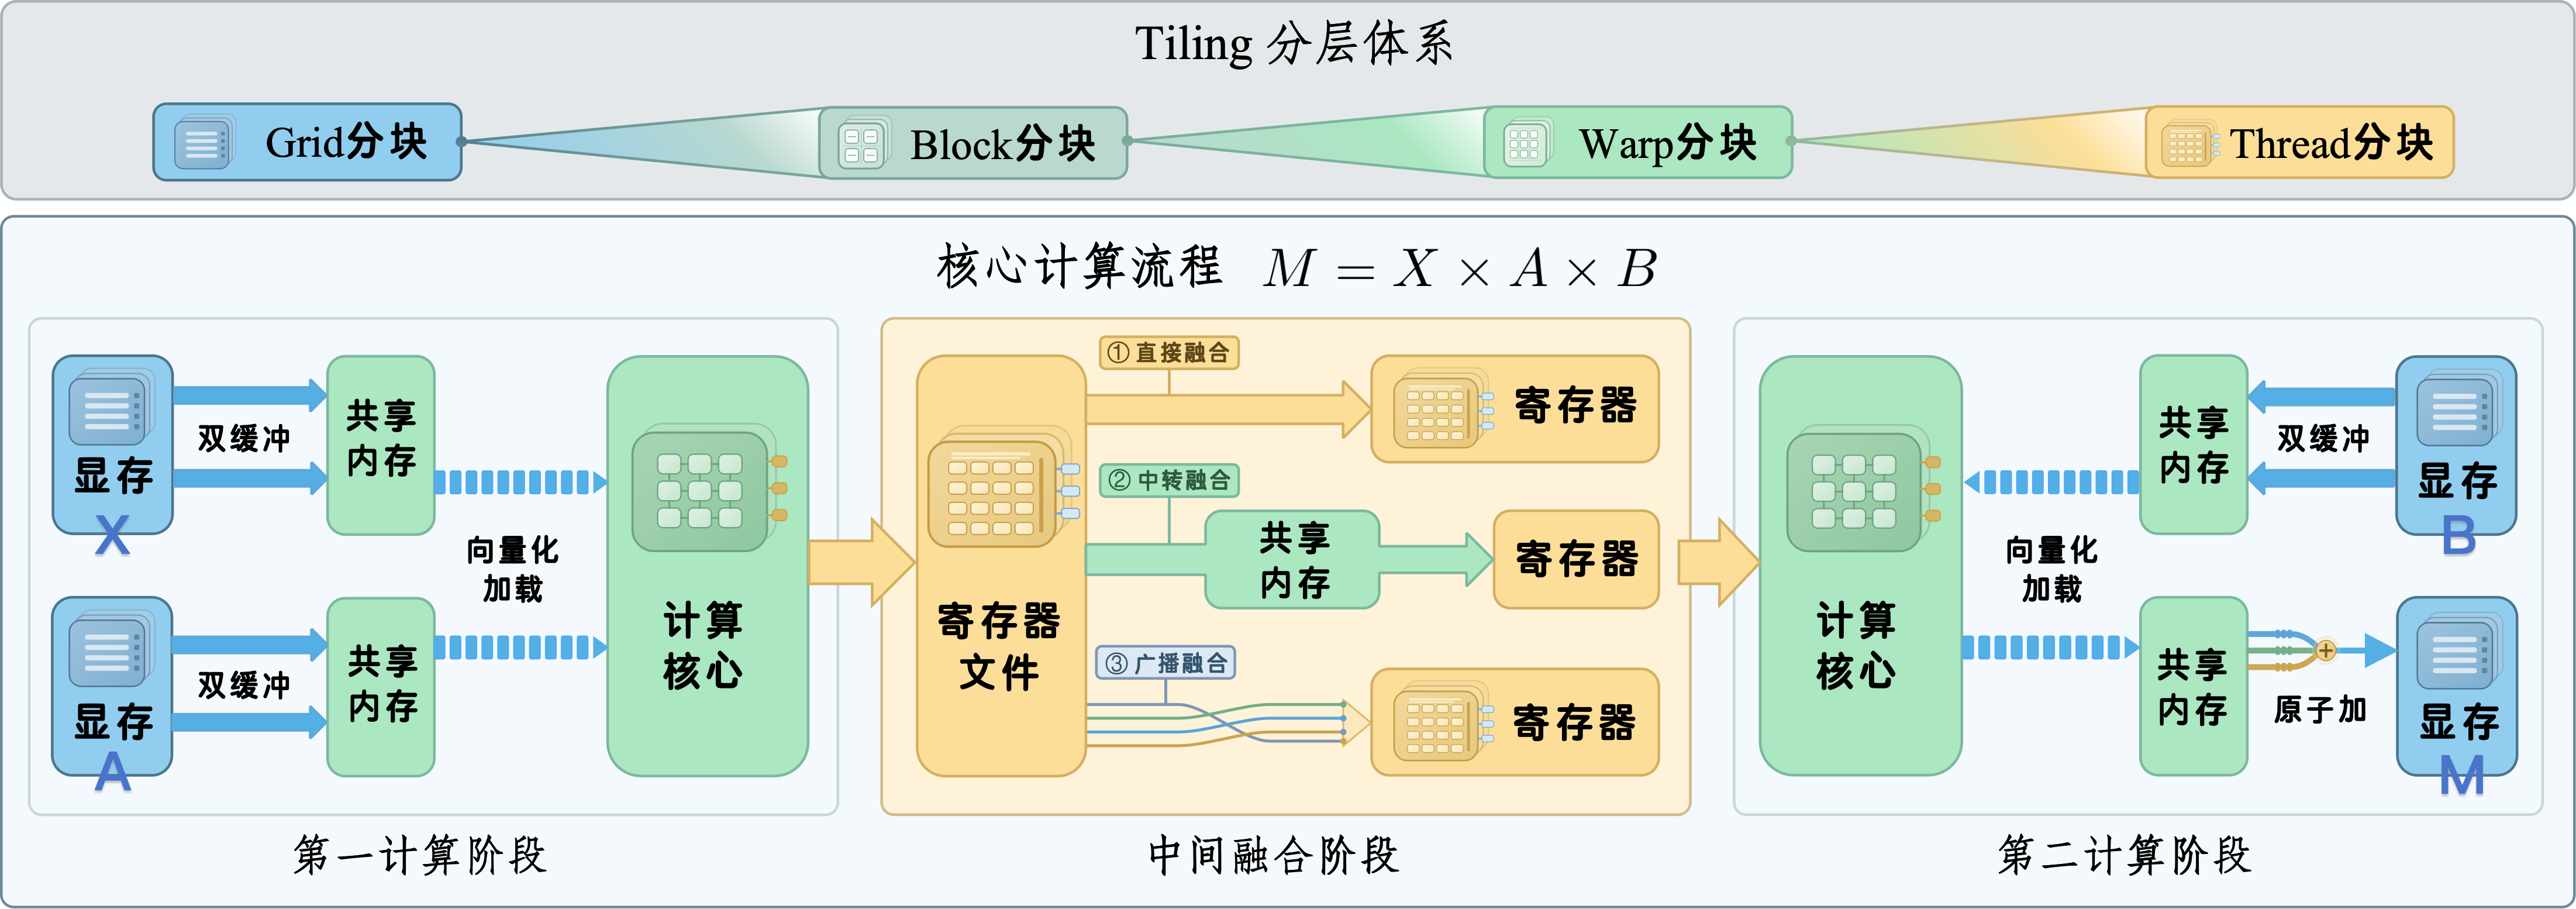
\includegraphics[width=\textwidth]{figures/trimm_framework.png}
    \caption{三矩阵融合算子的整体设计框架示例}
    \label{fig:trimm_framework}
\end{figure}

\subsection{融合思路示例}

示例主题中可以将融合策略简化为三类：寄存器转发、共享内存中转和面向 Tensor Core 的片段复用。这里不展开完整推导，只用少量内容占位，提醒使用者后续可按自己的论文需求继续细化。

    \section{融合算子的 CUDA 实现与优化}

\subsection{分块与任务映射}

若将三矩阵链式乘法映射到单个 kernel 中执行，通常需要同时考虑第一阶段生成中间结果与第二阶段消费中间结果的任务划分方式。这里保留一段简化描述，用于展示实现章节中的技术阐述风格。

\subsection{数据搬运优化}

融合实现通常需要关注三类数据路径：全局内存到共享内存、共享内存到寄存器，以及中间结果在片上存储之间的传递。实际写作中可在此扩展双缓冲、向量化加载、\texttt{cp.async} 或 \texttt{ldmatrix} 等实现细节。

\subsection{方法示例比较}

\begin{table}[htbp]
    \centering
    \caption{融合方法示例比较}
    \label{tab:fusion_method_compare}
    \renewcommand{\arraystretch}{1.25}
    \begin{tabular}{p{3.2cm}p{3.0cm}p{5.6cm}}
        \toprule
        方法 & 中间结果路径 & 说明 \\
        \midrule
        寄存器级数据广播 & 寄存器到寄存器 & 适合展示 warp 内数据交换与广播思路。 \\
        零中转数据转发 & Tensor Core 片段复用 & 适合展示寄存器片段兼容的设计思路。 \\
        梳状切片转储 & 共享内存中转 & 适合展示以共享内存换布局灵活性的方案。 \\
        \bottomrule
    \end{tabular}
\end{table}

表\ref{tab:fusion_method_compare} 仅作为表格排版示例。若你的论文并非 GPU 方向，可以直接用自己的实验表或方法表替换本节内容。

    \section{实验设计与性能评测}

\subsection{实验设置}

本模板仅保留少量实验章节内容，用于展示实验部分的标题层级、表格样式和说明文字布局。真实论文中，可在此补充硬件平台、软件版本、数据集和对比方法等信息。

\subsection{评测指标}

如果沿用三矩阵主题，可以将吞吐量、执行时间和显存访问开销作为指标；如果研究方向不同，则将本节替换为对应任务的评价指标即可。

\subsection{结果展示占位}

\begin{table}[htbp]
    \centering
    \caption{实验结果展示占位示例}
    \label{tab:experiment_placeholder}
    \begin{tabular}{ccc}
        \toprule
        方法 & 指标 1 & 指标 2 \\
        \midrule
        基线实现 & 待补充 & 待补充 \\
        融合实现 & 待补充 & 待补充 \\
        \bottomrule
    \end{tabular}
\end{table}

表\ref{tab:experiment_placeholder} 用于展示模板中的实验表格效果，正式使用时请将占位内容替换为自己的实验结果。

    \section{总结与展望}

本模板已经同步为当前项目使用的版式结构，并将正文示例压缩为少量三矩阵相关内容，主要用于占位和预览排版效果。

实际撰写时，建议保留章节组织、封面样式和参考文献配置，再逐步替换为自己的论文内容。若后续需要扩展附录、符号表或更多章节，也可以在当前结构基础上继续添加。


\bibliography{ref}

    \newpage

    \addcontentsline{toc}{nonumbersection}{致谢}
    \begin{center}
        {\zihao{-3}\heiti 致谢}
    \end{center}

    此处填写致谢内容。模板仓库中的文字仅用于展示排版位置，提交前请替换为自己的正式内容。

\end{document}
